\documentclass[english,12pt,twoside,a4paper]{article}
\usepackage[semibold]{sourcesanspro}
\usepackage[utf8]{inputenc}
\usepackage{mathpazo}
\usepackage{sectsty}
\usepackage[english]{babel}
\usepackage[T1]{fontenc}
\usepackage{fancyhdr}
\usepackage{xcolor} % où xcolor selon l'installation
\usepackage{scrextend} % Forcer la 4eme  de couverture en page pair
\usepackage{multirow} %% Pour mettre un texte sur plusieurs rangées
\usepackage[absolute]{textpos} 
\usepackage{graphicx, wrapfig}
\usepackage{geometry}
\usepackage{hyperref}
\usepackage{titlesec}
\usepackage{ulem, contour}
\usepackage{array}
\usepackage{tikz}
\usepackage{multicol, multicolrule}
\usepackage{caption, subcaption}
\usepackage{booktabs}
\usepackage{listings}
\usepackage{adjustbox}
\usepackage[indent=20pt]{parskip}
\usepackage{courier}
\usepackage{nameref}
\usepackage{lastpage}
\usepackage{blindtext}

\definecolor{Valentia}{RGB}{233,78,82}
\definecolor{Titleblue}{RGB}{114, 146, 162}

\SetMCRule{extend-fill=false}

\graphicspath{{./img}, {../img}}

\pagestyle{fancy}
\fancyhf{}
\fancyheadoffset{0.005\textwidth}
\fancyhead[LE,RO]{\slshape \rightmark}
\fancyhead[LO,RE]{\slshape \leftmark}
\lfoot{My Chief Cook Use Cases Analysis}
\rfoot{Page \thepage\ of \pageref*{LastPage}}

\definecolor{black}{rgb}{0,0,0}
\definecolor{green}{rgb}{0,0.5,0}
\definecolor{red}{rgb}{1,0,0}
\definecolor{blue}{rgb}{0,0,1}
\hypersetup{
	colorlinks=true,
	breaklinks=true,
	linkcolor=black,
	urlcolor=cyan,
	pdftitle={My Chief Cook Use Cases Analysis}}

\definecolor{codegreen}{rgb}{0,0.6,0}
\definecolor{codegray}{rgb}{0.5,0.5,0.5}
\definecolor{codepurple}{rgb}{0.58,0,0.82}
\definecolor{backcolour}{rgb}{0.95,0.95,0.95}
\lstdefinestyle{myStyle}{
  backgroundcolor=\color{white},   % choose the background color
  basicstyle=\footnotesize,        % the size of the fonts that are used for the code
  breakatwhitespace=false,         % sets if automatic breaks should only happen at whitespace
  breaklines=true,                 % sets automatic line breaking
  captionpos=b,                    % sets the caption-position to bottom
  commentstyle=\color{codegreen},    % comment style
  deletekeywords={...},            % if you want to delete keywords from the given language
  escapeinside={\%*}{*)},          % if you want to add LaTeX within your code
  extendedchars=true,              % lets you use non-ASCII characters; for 8-bits encodings only, does not work with UTF-8
  firstnumber=1,                   % start line enumeration with line 1
  frame=tb,                        % adds a frame around the code
  framerule=0.25pt,                % frame thickness
  keepspaces=true,                 % keeps spaces in text, useful for keeping indentation of code (possibly needs columns=flexible)
  keywordstyle=\color{blue},       % keyword style
  language=java,                   % the language of the code
  gobble=2,                        % the number of blank spaces before code
  morekeywords={},                 % if you want to add more keywords to the set
  numbers=left,                    % where to put the line-numbers; possible values are (none, left, right)
  numbersep=5pt,                   % how far the line-numbers are from the code
  numberstyle=\tiny\color{black},  % the style that is used for the line-numbers
  rulecolor=\color{black},         % if not set, the frame-color may be changed on line-breaks within not-black text (e.g. comments (green here))
  showspaces=false,                % show spaces everywhere adding particular underscores; it overrides 'showstringspaces'
  showstringspaces=false,          % underline spaces within strings only
  showtabs=false,                  % show tabs within strings adding particular underscores
  stepnumber=1,                    % the step between two line-numbers. If it's 1, each line will be numbered
  stringstyle=\color{codepurple},  % string literal style
  tabsize=2,                       % sets default tabsize to 2 spaces
}

\lstset{style=myStyle}

\renewcommand{\ULdepth}{1.8pt}
\contourlength{0.8pt}

\newcommand{\ul}[1]{%
	\uline{\phantom{#1}}%
	\llap{\contour{white}{#1}}%
}

\renewcommand{\footrulewidth}{1pt}
\captionsetup{labelfont={it, bf}, textfont={it}}
\urlstyle{same}

\newcommand{\resizeW}[1]{\resizebox{\linewidth}{!}{#1}}

\newcommand{\image}[4]{
  \begin{figure}[ht]
    \centering
    \fbox{\includegraphics[width=#2\linewidth]{#1}}
    \caption{#3}
    \label{fig:#4}
  \end{figure}
}

\newcommand{\usecasedesc}[7]{
  \subsection{#1}
  \subsubsection{Brief description}
  #2
  \subsubsection{Flow of events}
  #3
  \begin{multicols}{2}
    \subsubsection{Special requirements}
    #4
    \subsubsection{Preconditions}
    #5
    \subsubsection{Postconditions}
    #6
    \subsubsection{Extension points}
    #7
  \end{multicols}
}

\newcommand{\usecase}[3]{
  \fbox{%
    \parbox{0.3\linewidth}{%
      \centering
      \textbf{#1}\\
      \vspace{0.5em}
      \textit{Assignee : #2}\\
      \textit{Complexity : #3/5}
    }%
  }%
}
%%%%%%%%%%%%%%%%%%%%%%%%%%%%%%%%%%%%%%%%%%%%%%%%%%%%%%%%%%%%%%%

% \titleformat{\section}
% {\titlerule
% \vspace{.8ex}%
% \Large\bfseries}
% {\thesection.}{.5em}{}

% \titleformat{\part}[display]
% {\bfseries\Large}
% {\filleft PARTIE \Huge\thepart}
% {0ex}
% {\titlerule
% \vspace{1ex}%
% \filright}
% [\vspace{1ex}%
% \titlerule]

\captionsetup{labelfont={it, bf}, textfont={it}}
\setlength{\headheight}{15pt}
\setcounter{tocdepth}{2}

\begin{document}

\begin{titlepage}

  \newgeometry{left=2.5cm, bottom=3cm, top=2cm, right=2.5cm}

  \tikz[remember picture,overlay] \node[opacity=0.2,inner sep=0pt] at (73mm, -105mm){
\includegraphics[scale=1.5]{logo-2x.png}};

  {\fontfamily{phv}\fontseries{mc}\selectfont
  %*****************************************************
  %******************** TITRE **************************
  %*****************************************************
  \centering
  \color{Valentia}
  \fontsize{18}{13}\selectfont
  \textbf{My Chief Cook}

  \normalsize
  \color{black}

  \bigskip
  \textbf{Informatique et Gestion}

  \bigskip
  \textbf{Polytech Montpellier}

  \bigskip

  \color{Titleblue}
  \fontsize{17}{20.4}\selectfont
  \vspace{4cm}
  \textbf{USE CASES ANALYSIS}\\

  %*****************************************************

  \vspace{4cm}
  \fontsize{15}{18}\selectfont
  \color{black}
  \bigskip

  \vspace{2cm}
  \normalsize
  \textbf{Présenté par}\\
  \bigskip
  \fontsize{10}{12}\selectfont
  \vspace{1.5mm}
  \begin{table}[h]
    \centering
    \begin{tabular}{p{8cm}r}
      \toprule
      \textbf{[Corentin Clément]}      & \textbf{[Lead, Analytics]}          \\
      \textbf{[Alexis Fondard Martin]} & \textbf{[Development, Tests]}       \\
      \textbf{[Anais Velcker]}         & \textbf{[Documentation, Use cases]} \\
      \textbf{[Richard Martin]}        & \textbf{[Graphical User Interface]} \\
      \textbf{[Lucas Nouguier]}        & \textbf{[Database, Reports]}        \\
      \bottomrule
    \end{tabular}
  \end{table}

  %************************************
  %**  LOGO  UNIVERSITÉ
  %*****************************************************
  \vspace{\fill}
  \begin{center}
    
\includegraphics[height=60px]{LogoPolytech.png}
    \hfill
    
\includegraphics[height=65px]{LogoUM.png}
  \end{center}
  }
\end{titlepage}

%%%%%%%%%%%%%%%%%%%%%%%%%%%%%%%%%%%%%%%%%%%%%%%%%%%%%%%%%%%%%%
\newgeometry{top=2cm, bottom=2.5cm, left=2cm, right=2cm}
\setlength{\columnsep}{1cm}
\tableofcontents
\clearpage

\hypersetup{linkcolor=red}

\section{Problem Statement}
\subsection{Context}
You have been tasked by a start-up with building a proof of concept of their new cooking application. They need a prototype to show to investors and potential customers. The application will be used by Administrators to manage their recipes (and their inventory). The application will also be used by customers to search for recipes and eventually wines to come with their meal.
\subsection{Problem}
The final system will be an interactive web app, but for the proof of concept, you will be building a desktop application capable of running on any devices. It will allow Administrators to expose their recipes and partners while users will be able to order meals and wines. The application will also be able to suggest recipes based on the ingredients available in the user's fridge. Once they’ve made their choices, they must be able to pass command to either the restaurants, either to partners if they want to buy ingredients. They should as well receive wine recommandations if they chose to. Users will launch this prototype locally on their computer. For security and consistency reasons, some features will require some permissions (such as moderation).

For a more pleasant user experience, we’ll need users to be able to create “favorite lists” which must be name and where they can add recipes to easily find later. They must have full ownership of these lists. There will also be a feature to allow users to manage their meal plan up until 3 weeks ahead. They will be able to choose recipes and place them as a midday or evening meal. From the calendar users must be able to see the ingredient shopping list and the calendar should be persistent and auto-update according to the current date (for instance by strike-through past meals).

Users can send feedbacks too, by rating and commenting recipes. To promote helpful comments, there will a be voting system for comments (upvote/downvote) and comments with a high score (lots of upvotes) will be among the first comment in the list, whereas comments with low score (lots of downvotes) will be among the last. In addition, They should be able to suggest new recipes to Administrators by giving a description of what they think about (and eventually a name). Administrators will then be able to accept or reject the suggestion.

Administrators should be able to add to announcements to their page and manage them (update, hide, delete…). An announcement may have some labels to facilitate the search at a latter point

\subsection{Constaints}
Users should not be forced to expose their private life, so the system will retain as few information as possible :
\begin{itemize}
  \item Mandatory fields : their username, email address, password, secret question
  \item Optional fields : name, address, gender, birthday, phone
\end{itemize}

\noindent
Yet, Administrators must provide each fields for transparency. Also, some features will required optional fields to be fulfilled, so user must be warned when some fields are missing.

\subsection{Core Features}
\begin{itemize}
  \item Chose a recipe from ingredients and eventually auto-ajust proportions to match
        \begin{itemize}
          \item the number of people
          \item the number of meals
          \item the current quantity of ingredients in the fridge
        \end{itemize}
  \item Optionally add wine to the meal
  \item Make a meal plan for at most the next 3 weeks
  \item Redirect to partners' website to buy ingredients and/or wines
\end{itemize}

\section{Use Cases Model}
\image{usecase.png}{0.65}{Use Cases Model}{usecasesModel}
\vfill
\pagebreak
\section{Use Cases Estimated Complexity}

\noindent
\usecase{Manage profile}{Anaïs V.}{5}
\usecase{Manage recipe lists}{Richard M.}{2}
\usecase{Manage cart}{Richard M.}{3}

\noindent
\usecase{Manage recipes}{Lucas N.}{4}
\usecase{Manage ingredients}{Lucas N.}{2}
\usecase{Manage categories}{Corentin C.}{1}

\noindent
\usecase{Manage comments}{Alexis F.}{3}
\usecase{Manage suggestions}{Corentin C.}{3}
\usecase{Manage calendar}{Alexis F.}{3}

\noindent
\usecase{Manage news}{Anaïs V.}{2}
\usecase{Manage partners}{Richard M.}{1}
\usecase{Manage advertisement}{Corentin C.}{2}

\section{Use Cases Description}
\usecasedesc
{Ingredient management \label{sec:ingredientManagement}}
{
  Ingredients are the base of recipes. As for recipes, they can be modified (created, updated, deleted) by Administrators only. They will be able to specify a name, a list of tags (categories) and wether it's allergen or not. If it's allergenic, it must be emphasized. Name, and allergen status are mandatory fields.

  Administrators should be able to search ingredients by name and the result should be sorted by name by default. They should be able to sort by tags, and allergenic status. Results should be paginated and the number of results per page should be configurable. They should also be able to filter by tags and allergenic status.

  \image{ingredientManagement}{0.75}{Ingredient Management}{ingredientManagement}
}
{
  This Use Case starts whenever a Administrator wants to add, update or delete an ingredient to the database

  \paragraph{Basic Flows}
    \begin{itemize}
      \item Create an ingredient : The system asks the Administrator to enter the information about the ingredient : name, tags (categories), allergen 
      \begin{enumerate}
        \item Once the Administrator provided at least the required information, the system adds the ingredient to the database.
        \item The system provide a success message, returns the newly created ingredient, and goes back to ingredient management menu.
      \end{enumerate}
      \item Update an ingredient : The system ask the Administrator to enter  the new information about the ingredient
      \begin{enumerate}
        \item Once the Administrator provided at least the required information, the system updates the ingredient in the database.
        \item The system provide a success message, updates the ingredient on the application, and goes back to ingredient management menu.
      \end{enumerate}
      \item Delete an ingredient : The system ask the Administrator which ingredient he wants to delete
      \begin{enumerate}
        \item Once the Administrator chosed the ingredient, the system checks if it is used by any recipe. If it is not, the system deletes the ingredient from the database.
        \item The system provide a success message, deletes the ingredient on the application, and goes back to ingredient management menu.
      \end{enumerate}
    \end{itemize}
  \paragraph{Alternative Flows}
  \begin{itemize}
    \item Create an ingredient :
    \begin{enumerate}
      \item If the Administrator does not provide every mandatory fields and tries to validate, the system display an error message as a "toast" and does nothing else.
      \item If the Administrator cancels, the system goes back to ingredient management menu.
    \end{enumerate}
    \item Update an ingredient :
    \begin{enumerate}
      \item If the Administrator does not provide every mandatory fields and tries to validate, the system display an error message as a "toast" and does nothing else.
      \item If the Administrator tries to update an ingredient already use by a recipe, the system display a warning message and ask for confirmation. If the Administrator confirms, the system updates the ingredient in the database and in the app and the normal flow continues. If the Administrator does not confirm, the system does nothing else.
      \item If the Administrator cancels, the system goes back to ingredient management menu.
    \end{enumerate}
    \item Delete an ingredient :
    \begin{enumerate}
      \item If the Administrator tries to delete an ingredient already use by a recipe, the system display a error message. Otherwise, the system deletes the ingredient in the database and in the app and the normal flow continues.
      \item If the Administrator cancels, the system goes back to ingredient management menu.
    \end{enumerate}
  \end{itemize}
}
{Must be thread-safe in case multiple Administrators are modifying the same ingredient.}
{The Administrator must be logged onto the system before this use case begins.}
{If it's successful, the ingredient will be added/updated/deleted from the database. Otherwise, the state remains unchanged.}
{None}

\usecasedesc
{Recipe management \label{sec:recipeManagement}}
{
  Recipes can be modified (created, updated, deleted) by Administrators only. They will be able to specify a name, a summary, a list of ingredients, some categories, a description, and maybe a picture of it. Recipes can be search by name, tags, ingredients, whether it contains allergens or not, and may be sorted by name or popularity.
  
  If a recipe contains allergens, it must be specified and allergenic ingredients must appear in emphasized text. A recipe can also receive many comments and ratings from the users.

  \image{recipeManagement}{0.75}{Recipe Management}{recipeManagement}
}
{
  This Use Case starts when a Administrator wants to add, update or delete a recipe to the database.

  \paragraph{Basic Flows}
  \begin{itemize}
    \item Create a recipe : The system asks the Administrator to enter the information about the recipe : name, summary, tags (categories), ingredients, description, picture
    \begin{enumerate}
      \item Once the Administrator provided at least the required information, the system adds the recipe to the database.
      \item The system provide a success message, returns the newly created recipe, and goes back to recipe management menu.
    \end{enumerate}
    \item Update a recipe : The system ask the Administrator to enter the new information about the recipe
    \begin{enumerate}
      \item Once the Administrator provided at least the required information, the system updates the recipe in the database.
      \item The system provide a success message, updates the recipe on the application, and goes back to recipe management menu.
    \end{enumerate}
    \item Delete a recipe : The system ask the Administrator which recipe he wants to delete
    \begin{enumerate}
      \item Once the Administrator chosed the recipe, the system deletes the recipe from the database.
      \item The system provide a success message, deletes the recipe on the application, and goes back to recipe management menu.
    \end{enumerate}
  \end{itemize}
  \paragraph{Alternative Flows}
  \begin{itemize}
    \item Create a recipe :
    \begin{enumerate}
      \item If the Administrator does not provide all the mandatory information and tries to validate, the system display an error message as a "toast" and does nothing else.
      \item If the Administrator cancels, the system goes back to recipe management menu.
    \end{enumerate}
    \item Update a recipe :
    \begin{enumerate}
      \item If the Administrator does not provide all the mandatory information and tries to validate, the system display an error message as a "toast" and does nothing else.
      \item If the Administrator cancels, the system goes back to recipe management menu.
    \end{enumerate}
    \item Delete a recipe :
    \begin{enumerate}
      \item If the Administrator cancels, the system goes back to recipe management menu.
    \end{enumerate}
  \end{itemize}
}
{Must be thread-safe in case multiple Administrators are modifying the same recipe.}
{The Administrator must be logged onto the system before this use case begins.}
{If it's successful, the recipe will be added/updated/deleted from the database. Otherwise, the state remains unchanged.}
{None}
\usecasedesc{Category Management \label{sec:categoryManagement}}
{
  A recipe belongs to one or more categories. The goal is to give simple information about the recipe (for example, the recipe is a "vegetarian" "dish"), but also to be able to apply filters on the recipe search.
  
  The different categories can be created, modified and deleted only by administrators connected to their account.

  \image{categoryManagement}{0.75}{Category Management}{categoryManagement}
}
{
  The system requests that the Administrator specify the function he/she would like to perform : either Add a Category, Update a Category, or Delete a Category (see \autoref{fig:categoryManagement}). Once the Administrator provides the requested information, one of the sub flow is executed.

  \paragraph{Basic Flows}
    \begin{itemize}
      \item If the Administrator selected "Add a Category", the Add a Category sub flow is executed :
      \begin{enumerate}
        \item The system request that the administrator enter new information. This include the name’s category.
        \item the system generates a id number for the new category, register it in the database, the category is available for recipes and the administrator is informed that the creation worked with the message "The category has been created".
      \end{enumerate}
      \item If the Administrator selected "Update a Category", the Update a Category sub flow is executed :
      \begin{enumerate}
        \item The administrator selects a category from the list of categories (obtained from the system). The administrator can only change the name’s category.
        \item The system update the category’s name in the database. The administrator is informed that the update worked with the message "The category has been updated".
      \end{enumerate}
      \item If the Administrator selected "Delete a Category", the Delete a Category sub flow is executed :
      \begin{enumerate}
        \item The administrator selects a category from the list of category (obtained from the system). The administrator can delete the chosen category and need to confirm to delete. 
        \item The system update the database therefore deletes the category. The administrator is informed that the delete has worked with the message "The category has been deleting".
      \end{enumerate}
    \end{itemize}

  \paragraph{Alternate Flows}
  \begin{itemize}
    \item Add Category or Update category with an existing name : the administrator can’t create a category or update a category with an existing name. In this case, the state will not change and the administrator is notified that he is not allowed to do the change/creation with a message "This name is already use".
    \item Action cancelling : If the Administrator decides to cancel the current action, then the action aborts and the system is unchanged.
  \end{itemize}
}
{
  None
}
{
  The Administrator must be logged onto the system before this use case begins.
}
{
  If the use case was successful, the category information is added, updated, or deleted from the system. Otherwise, the system state is unchanged.
}
{
  None
}

\usecasedesc{
  Ad management \label{sec:adManagement}
}
{
  We have advertisements in the application, to suggest to buy some ingredients with a promotion with our partners. So we need to manage the ads : create an ad, update an ad and delete an ad.

  The different adverts can be created, modified and deleted only by administrators connected to their account.

  \image{adManagement.png}{0.75}{Ad Management}{adManagement}
}
{
  The system requests that the Administrator specify the function he/she would like to perform : Add an Advert, Update an Advert, or Delete an Advert (see \autoref{fig:adManagement}). Once the Administrator provides the requested information, one of the sub flows is executed.

  \paragraph{Basic Flows}
  \begin{itemize}
    \item If the Administrator selected “Add an Advert“, the Add an Advert sub flow is executed :
    \begin{enumerate}
      \item The system request that the administrator enter new information. This include the  partner, the product, the promotion, the price.
      \item The system generates a id number for the new advert, register it in the database and the ad is available for the ingredient. The administrator is informed that the creation worked with the message “The advert has been created”.
    \end{enumerate}
    \item If the Administrator selected “Update a Category“, the Update an Advert sub flow is executed :
    \begin{enumerate}
      \item The administrator selects an ad from the list of adverts (obtained from the system). The administrator can change the  partner, the product, the promotion, the price.
      \item The system updates the data in the database and the administrator is informed that the update worked with the message “The advert has been updated”.
    \end{enumerate}
    \item If the Administrator selected “Delete a Category“, the Delete an Advert sub flow is executed :
    \begin{enumerate}
      \item The administrator selects an ad from the list of adverts (obtained from the system). The administrator can delete the chosen advert and need to confirm to delete.
      \item The system updates the database therefore deletes the ad. The administrator is informed that the delete worked with the message “The advert has been deleted”.
    \end{enumerate}
  \end{itemize}

  \paragraph{Alternate Flows}
  \begin{itemize}
    \item Action cancelling : If the Administrator decides to cancel the current action, then the action aborts and the system is unchanged.
  \end{itemize}
}
{
  None
}
{
  The Administrator must be logged onto the system before this use case begins.
}
{
  If the use case was successful, the advertising information is added, updated, or deleted from the system. Otherwise, the system state is unchanged.

}
{
  None
}

\usecasedesc
{
  Suggestion Management \label{sec:suggestionManagement}
}
{
  When the customer uses the application, he can sometimes be disappointed because he can’t find a recipe or an ingredient or want to suggest a new feature for the application. The manage suggestions is the CRUD to this. The users will create suggestions and the admins will read, update and delete or implement the suggestion.

  \image{suggestionManagement.png}{0.65}{Suggestion Management}{suggestionManagement}
}
{
  The functionality is available through a button placed in different places in the application. The button to access the suggestion form page is visible in the drop down menu and when searching for an ingredient or recipe the button is directly available on the page if no results match the user's search.

  \pagebreak

  \paragraph{Basic Flows}
  \begin{itemize}
    \item If the Payroll User selected “Propose a Suggestion“, the Add a Suggestion sub flow is executed :
    \begin{enumerate}
      \item The customer enters the information on the system. This includes the category of the suggestion (ingredient, recipe, feature) and a text field to detail the request (the name of the ingredient or the new feature requested\dots).
      \item The system generates a id number for the new suggestion, register it in the data-base and the suggestion is available for admins. The customer is informed that the creation worked with the message “The suggestion has been sent”.
    \end{enumerate}
    \item If the Administrator selected “Update a Suggestion“, the Update a Suggestion sub flow is executed :
    \begin{enumerate}
      \item The administrator selects a suggestion from the list of suggestion (obtained from the system). The admin can change the suggestion, that is change the text field and the category of the suggestion if the customer is mistaken.
      \item The system updates changes in the database. The administrator is informed that the update worked with the message “The suggestion has been updated”.
    \end{enumerate}
    \item If the Administrator selected “Delete a Suggestion“, the Delete a Suggestion sub flow is executed :
    \begin{enumerate}
      \item The administrator selects a suggestion from the list of suggestion (obtained from the system). The administrator can delete the chosen suggestion and need to confirm to delete.
      \item The system updates the database therefore deletes the ad. The administrator is informed that the delete worked with the message “The advert has been deleted”.
    \end{enumerate}
  \end{itemize}

  \paragraph{Alternate Flows}
  \begin{itemize}
    \item Action cancelling : If the Administrator decides to cancel the current action, then the action aborts and the system is unchanged.
  \end{itemize}
}
{None}
{The Administrator must be logged onto the system before this use case begins.}
{If the use case was successful, the advert information is added, updated, or deleted from the system. Otherwise, the system state is unchanged.}
{None}
\usecasedesc{Comment management}
{
  This use case describes how a User can see comments and rates, post a comment under a recipe and/or rate a recipe. An Admin can also manage all comments (a kind of moderation, he can delete a comment if he thinks there is an abuse).

  \image{commentManagement}{0.75}{Comment management}{commentManagement}
}
{
  \begin{multicols}{2}
    This use case starts when the User wishes to comment or rate a recipe.
    \begin{itemize}
      \item The User opens a recipe and scrolls down to the Comment section below.
      \item There he can see the average rate and read all comments, that contain each a rate of the recipe.
      \item If the User clicks on the stars button (to rate the recipe), the Add Comment sub flow is executed.
    \end{itemize}

    \columnbreak
  
    This use case can also start when the Admin is on his moderation section.
    \begin{itemize}
      \item The Admin opens the list of comments, or goes to a recipe and scrolls down to the Comment section.
      \item If the Admin clicks on the Delete Comment button, the Delete Comment sub flow is executed.
    \end{itemize}
  \end{multicols}

  \paragraph{Basic Flows}
  \begin{itemize}
    \item Add Comment :
    \begin{enumerate}
      \item The User has clicked on the stars button (he selected a note between 1-5 stars), then he can possibly fill the form bellow. This form includes:
      \begin{itemize}
        \item Name of the comment (optional)
        \item Content of the comment (optional but need a name)
      \end{itemize}
      \item The User needs to click on the Submit button to send the comment.
    \end{enumerate}
    \item Delete comment :
    \begin{enumerate}
      \item The Admin clicks on the Delete Comment button. A new popup appears asking the Admin if he is sure of his decision.
      \item The Admin clicks on the Validate button, then the selectionned button is deleted.
    \end{enumerate}
  \end{itemize}

  \paragraph{Alternative Flows}
  \begin{itemize}
    \item Delete canceled : if in the Delete Comment sub flow the Admin decides not to delete the comment, the delete is canceled and the Basic Flow is restarted at the beginning.
  \end{itemize}
}
{None}
{The User/Admin needs to be logged in and a recipe needs to be created before this use case begins.}
{If the use case was successful, the comment is added/modified and the other users can now see the new/modified comment. If the Admin has removed the comment, it’s now no longer visible.
}
{None}

\usecasedesc{Calendar management}
{
  This use case describes how a User can save his recipes in a calendar and plan when to make them. He can see his calendar whenever he needs to, and delete a recipe from the calendar if he needs to.

  \image{calendarManagement}{0.75}{Calendar management}{calendarManagement}
}
{
  This use case starts when the User wishes to add a recipe to his calendar or see it :
  \begin{enumerate}
    \item The User opens a recipe or the list of recipes.
    \item If the User clicks on the Add to Calendar button (which can be seen on a recipe or on each recipe of the list), the Add to Calendar sub flow is executed.
    \item If the User clicks on the calendar button/icon, he can see his calendar with all his recipes saved in it.
    \item If the User clicks on the cross (X) of a recipe saved in his calendar, the Delete from Calendar sub flow is executed.
  \end{enumerate}

  \paragraph{Basic Flows}
  \begin{itemize}
    \item Add to calendar :
    \begin{enumerate}
      \item The User clicks on the Add to Calendar button, then a calendar popup is shown and ask for the User to select a date (dd/mm/yyyy) and a meal (breakfast, lunch, dinner, snack, other).
      \item The User needs to click on the Validate button to save the recipe to this date.
    \end{enumerate}
    \item Delete from calendar : the User has clicked on the cross (X) of a recipe saved in his calendar, a Validate popup is shown to check if he really needs to delete the recipe saved for this day.
  \end{itemize}

  \paragraph{Alternative Flows}
  \begin{itemize}
    \item Add canceled : if in the Add to Calendar sub flow the User decides not to add the recipe, the saving is canceled and the Basic Flow is restarted at the beginning.
    \item Delete canceled : if in the Delete from Calendar sub flow the User decides not to delete the recipe, the delete is canceled and the Basic Flow is restarted at the beginning.
  \end{itemize}
}
{None}
{The User needs to be logged and a recipe needs to be created before this use case begins.}
{If the use case was successful, the recipe is added to the date in the calendar and the User can now see it in his calendar. Otherwise, the system state is unchanged.}
{None}
\usecasedesc{Recipe List}
{
  If the user whises to save a recipe, he can use the recipe lists. He can have multiple lists to better sort them (for instance seasonal recipes, or recipes for a specific occasion). There will be a default list named "Favorites". One user can't have two lists with the same name.

  \image{recipeListManagement}{0.75}{Recipe list management}{recipeListManagement}
}
{
  This use case begins when the user wants to access to his lists, either to modify them or read them

  \begin{itemize}
    \item If the user clicks on the "create a list", then the Create list sub flow is executed
    \item If the user clicks on a list, then the Display recipes sub flow is executed 
    \item If the user clicks on the "delete" button of a list, then the Delete list sub flow is executed
    \item If the user clicks on the "rename" button of a list, then the Rename list sub flow is executed
    \item If the user clicks on the "add to list" button of a recipe, then the Add to list sub flow is executed
    \item If the user clicks on the "remove from list" button of a recipe, then the Remove from list sub flow is executed
  \end{itemize}
  \paragraph{Basic Flows}
  \begin{itemize}
    \item Create lists :
    \begin{enumerate}
      \item The system ask the user to enter a name for the new list
      \item The system creates the list
      \item The system returns the newly created list to the user and displays it
    \end{enumerate}
    \item Display recipes : the system displays the recipes of the list. It may be displayed as a list or as a grid.
    \item Delete lists :
    \begin{enumerate}
      \item The system asks the user to confirm the deletion
      \item The system deletes the list and removes it from the application
    \end{enumerate}
    \item Rename list :
    \begin{enumerate}
      \item The system asks the user to enter a new name for the list
      \item The system renames the list in the database and in the application
    \end{enumerate}
    \item Add to list :
    \begin{enumerate}
      \item The system asks the user to select the list to which he wants to add the recipe
      \item The system adds the recipe to the list
    \end{enumerate}
    \item Remove from list : the system removes the recipe from the list
  \end{itemize}

  \paragraph{Alternative Flows}
  \begin{itemize}
    \item Remove recipe lists : if the user tries to delete a list that is not empty, the system asks him to confirm the deletion
    \item Create recipe list : if the user tries to create a list with a name that already exists, the system asks him to enter a new name
    \item Updating a list : if the user tries to update a list that doesn't exist, the system warns him with a popup
  \end{itemize}
}
{
  None
}
{
  The user must be logged in to access to his lists.
}
{
  If it’s successful, the lists will be added/updated from the database. Otherwise, the state remains unchanged.
}
{
  None
}

\usecasedesc{Cart management}
{
  The cart is a list of the recipe and ingredients an user ordered. There is only one cart by user and it cannot be deleted, only emptied. On the main page of the cart we'll be able to see the list of ordered recipes and ingredients. "Standalone" ingredients will appear separately from recipes' ingredients.

  \image{cartManagement}{0.95}{Cart management}{cartManagement}
}
{
  This use case begins when a user wants to either add an element to his cart, see his cart or empty it.

  \begin{itemize}
    \item If the user clicks on the "add to cart" button of a recipe or ingredient, then the Add element to cart sub flow is executed
    \item If the user clicks on the "remove from cart" button of a recipe or ingredient, then the Remove element from cart sub flow is executed
    \item If the user clicks on the "change quantity" button of a recipe or ingredient, then the Change quantity sub flow is executed
    \item If the user clicks on the "empty cart" button, then the Empty cart sub flow is executed
    \item If the user clicks on the "order" button, then the Order sub flow is executed
  \end{itemize}

  \paragraph{Basic Flows}
  \begin{itemize}
    \item Add element to cart :
    \begin{enumerate}
      \item The system asks the user for the quantity he wants
      \item The system adds the element to the cart
    \end{enumerate}
    \item Remove element from cart : the system removes the element from the cart
    \item Change quantity :
    \begin{enumerate}
      \item The system asks the user for the new quantity
      \item The system updates the quantity of the element in the cart
    \end{enumerate}
    \item Empty cart :
    \begin{enumerate}
      \item The system asks the user to confirm the emptying
      \item The system empties the cart
    \end{enumerate}
    \item Order :
    \begin{enumerate}
      \item The system asks the user to confirm the order. It displays the list of ordered recipes and ingredients and the lists of total quantities of ingredients needed.
      \item The system ask for the delivery address, phone and payement method. If the user has already entered this information, the system autocomplete the form.
      \item Once the user has provided the requested information, the system sends the order. For this proof of concept, it will juste be a message with the order information.
      \item The cart is emptied
    \end{enumerate}
  \end{itemize}

  \paragraph{Alternative Flows}
  \begin{itemize}
    \item Add element to cart :
    \begin{enumerate}
      \item The user wants to add an element that is already in his cart
      \item The system displays a message to inform him that the element is already in his cart, and launch the "Change quantity" sub flow.
    \end{enumerate}
    \item Empty cart : if the user can't clear his cart, for unknown reasons, a message is displayed to inform him that the cart can't be cleared.
  \end{itemize}
}
{None}
{The user must be logged in to access to his cart.}
{If it’s successful, the cart will be updated in the database. Otherwise, the state remains unchanged.}
{None}

\usecasedesc{Partner management}
{
  MyChiefCook has a list of Partner companies that are displayed to the users. They may offer discounts or special offers to the users. Users can access to the list of partners and their offers.

  \image{partnerManagement}{0.75}{Partner management}{partnerManagement}
}
{
  This use case begins when an admin wants to manage the list of partners.

  \begin{itemize}
    \item If the admin clicks on the "add partner" button, then the Add partner sub flow is executed
    \item If the admin clicks on the "delete partner" button, then the Delete partner sub flow is executed
    \item If the admin clicks on the "update partner" button, then the Update partner sub flow is executed
  \end{itemize}

  \paragraph{Basic Flows}
  \begin{itemize}
    \item Add partner :
    \begin{enumerate}
      \item The system asks the admin to enter the information about a partner (name, description, website) and their offers (description, discount)
      \item The system adds the partner to the database
    \end{enumerate}
    \item Edit partner :
    \begin{enumerate}
      \item The system asks the admin to enter the new information about the partner
      \item The system updates the partner in the database
    \end{enumerate}
    \item Delete partner :
    \begin{enumerate}
      \item The system asks the admin to confirm the deletion
      \item The system deletes the partner from the database
    \end{enumerate}
  \end{itemize}

  \paragraph{Alternative Flows}
  \begin{itemize}
    \item Add/Edit partner : if an admin tries to add a partner's offer on an ingredient on which there is already a discount, they system asks him to confirm the deletion of the previous offer and replace it with the new one.
    \item Operation canceled : if the admin cancels the operation, the modification are not saved and the admin is redirected to the partner management page.
  \end{itemize}
}
{None}
{The user must be logged in and be an admin}
{If it’s successful, the partner will be added/updated from the database. Otherwise, the state remains unchanged.}
{None}
\subusecasedesc{News management}
{
  The news will show the user what is new (change in the application, new recipes, new partner). It can be modified (created, updated) by administrators only. They will be able to specify a title, a description, and a picture if they want. They also will be able to display or not the news to the users.

  \image{newsManagement}{0.75}{News management}{newsManagement}
}
{
  This use case starts when the administrator wishes to add, change, and/or display a news from the system.

  The system requests that the administrator specify the function he/she would like to perform (either add a news, update a news or display a news). Once the administrator has provided the requested information, one of the sub flows is executed.

  \paragraph{Basic Flows}
  \begin{itemize}
    \item If the administrator selected "Add news", the Add news sub flow is executed :
    \begin{enumerate}
      \item The system requests that the administrator enter the news information. This includes : title, description, pictures (optional)
      \item Once the administrator has provided the requested information, the system generates and assigns a unique news id to the new news. The news is added to the system and the news display is set to "not displayed" by default.
    \end{enumerate}
    \item If the administrator selected "Update news", the Update news sub flow is executed :
    \begin{enumerate}
      \item The system requests that the administrator makes the desired changes to the news information. This includes any of the information specified in the Add a news sub-flow.
      \item Once the administrator has updated the necessary information, the system updates the news record with the updated information.
    \end{enumerate}
    \item If the administrator selected "Display news", the Display news sub flow is executed : the system requests that the administrator selects the option he wants. He can display the news to the users or hide it.
    
  \end{itemize}

}
{Must be thread-safe in case multiple administrators are modifying the news.}
{The administrator must be logged onto the system before this use case begins.}
{If it’s successful, the news will be added/updated from the database and display if the administrator wishes. Otherwise, the state remains unchanged.}
{None}


\section{User management}
This use case is a very big one and particularly important because it is the base of the application, which is the reason why it has been placed in a separate section.

\begin{figure}[h]
  \centering
  \begin{subfigure}{0.45\linewidth}
    \fbox{
      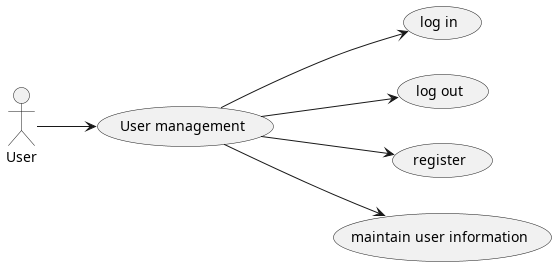
\includegraphics[width=0.94\linewidth]{userUserManagement}
    }
    \caption{Standard user}
  \end{subfigure}
  \hfill
  \noindent
  \begin{subfigure}{0.45\linewidth}
    \centering
    \fbox{
      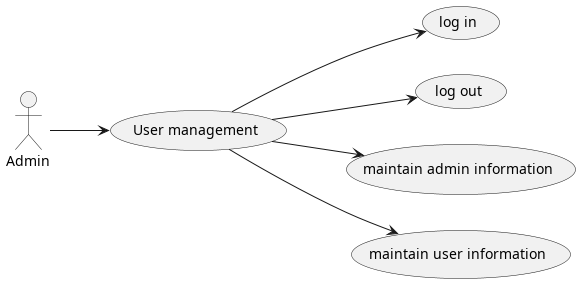
\includegraphics[width=0.92\linewidth]{adminUserManagement}
      }
    \caption{Administrator}
  \end{subfigure}
  \caption{User management}
\end{figure}
\subusecasedesc
{Logging in}
{
  Users can signin / signup to the application by providing their username, email, password, and optionally their name, address, social network accounts, gender, birthday and a picture.

}
{
  This starts when a user wishes to log into the application.

  \paragraph{Basic Flows}
  \begin{itemize}
    \item Signin : if the user selected "Sign in” the Sign in sub flow is executed. The system requests that the user enter the login information (email \& password). Then :
    \begin{enumerate}
      \item If the user provides the requested information, the system validates the entered information and logs the user into the system.
      \item If the user selects "forgot password”  the system will ask the secret question and if the system validates, the user is logged in and he can modify his password else, he is redirected to the login page.
      \item If the user selects "Register”, the user will be redirect to the Register flow.
    \end{enumerate}
  \end{itemize}

  \paragraph{Alternative Flows}
  \begin{itemize}
    \item Invalid email/password : if in the Have an account flow, the user enters an invalid email and/or password, the system displays an error message. The user can choose to either return to the beginning of the Have an account flow or cancel the login, at which point the use case ends.
    \item Login canceled : if in the sign in sub flow the user decides not to login, the signin is canceled and the user is redirected to the log in sub flow.
  \end{itemize}
}
{None}
{None}
{If the log in was successful, the user is now logged into the system.  If not, the system state is unchanged.}
{None}

\subusecasedesc
{Logging out}
{Users can also log out of the application}
{
  This starts when a user wishes to log out the application : the system logs out the user from the system.
}
{User must be logged in to log out}
{
  If the log out was successful, the user is now disconnected from the system and he will be redirected to the login page.
}
{None}
{None}

\subusecasedesc
{Register}
{When a new user wants to use the application}
{
  The system requests that the user enter the register information. This includes :
  \begin{itemize}
    \item Email / Password / Secret question / Answer (mandatory)
    \item Name
    \item Birthdate
    \item Phone
    \item Allergies
  \end{itemize}

  \paragraph{Basic Flows}
  Once the user has provided the requested information, the system validates the entered information, generates and assigns a unique user id to the user. The user is added to the system and logs into the system.
  \paragraph{Alternative Flows}
  \begin{itemize}
    \item Invalid form : if the user enters an email already used or if another field of the form is wrong, the system displays an error message ("Something went wrong” for instance).
    \item Registration canceled : if in the Register sub flow the user decides not to register, the register is canceled and the user is redirected to the login sub flow.
  \end{itemize}
}
{None}
{User should not already have an account.}
{If the register was successful, the user is redirected to the home page.}
{None}

\subusecasedesc
{Change information}
{
  This use case allows the user to maintain his personal information. This includes changing user information from the system. He can also ask for deleting his account.
}
{
  This use case begins when a user wants to change his information.

  The system requests that the user specify the function he/she would like to perform (either modify personal information or ask for deleting). Once the user has provided the requested information, one of the sub flows is executed

  \paragraph{Basic Flows}
  \begin{itemize}
    \item Change personal information : if the user selected "modify personal information", the modify personal information sub flow is executed :
    \begin{enumerate}
      \item The system retrieves his personal information and displays the user information. The user makes the desired changes to his information. This includes any of the information specified in the Register sub flow.
      \item Once the user has updated the necessary information, the system updates the user record with the updated information.
    \end{enumerate}
    \item Account deletion : If the user selected "Ask for deleting", the Ask for deleting sub flow is executed :
    \begin{enumerate}
      \item The system sends a notification to the administrator informing him that the user "X” wants to delete his account.
      \item The administrator can decide if he delete it or not. But as a GDPR compliant application, the administrator must delete the account if the user asks for it.
    \end{enumerate}
  \end{itemize}

  \paragraph{Alternative Flows}
  \begin{itemize}
    \item Modify personal information canceled : if in the modify personal information sub flow and the user decides not to modify his information, the modification is canceled and the user is redirected to the user page.
    \item Ask for deleting canceled : if in the ask for deleting sub flow and the user decides not to delete his account, the demand is canceled he is redirected to the user page.
  \end{itemize}
}
{None}
{User must be loggged in}
{If the use case was successful, the user information is updated from the system.  Otherwise, the system state is unchanged.}
{None}

\subusecasedesc
{Administrator}
{
  This use case allows the administrator to maintain his personal information and maintain users. This includes changing his personal information from the system. He can also view the list of users and delete user account.
}
{
  The system requests that the administrator specify the function he/she would like to perform (either modify personal information or deleting).

  \paragraph{Basic Flows}
  \begin{itemize}
    \item If the administrator selected "modify personal information", the modify personal information subflow is executed :
    \begin{enumerate}
      \item The system retrieves his personal information and displays the administrator information.
      \item The administrator makes the desired changes to his information. This includes any of the information specified in the Register sub flow.
      \item Once the administrator has updated the necessary information, the system updates the user record with the updated information.
    \end{enumerate}
    \item If the administrator selected "view all users", the view user sub flow is executed :
    \begin{enumerate}
      \item The system retrieves the list of all users and displays it. The administrator has the list of all users.
      \item He can click and see all the information of a user.
    \end{enumerate}
    \item If the administrator selected "Delete a user ", the Delete a user sub flow is executed :
    \begin{enumerate}
      \item The administrator receive a notification that a user wants to delete his account.
      \item He decide to delete the account permanently or not (GDPR).
      \item If he decides to delete the account, an email will be sent to the user and the system updates the user record.
    \end{enumerate}

  \end{itemize}
  \paragraph{Alternative Flows}
  \begin{itemize}
    \item Modify personal information canceled : if in the modify personal information sub flow the administrator decides not to modify his information, the modification is canceled and the administrator is redirected to the user page.
  \end{itemize}

}
{None}
{The administrator must be logged in.}
{
  If it was successful, the information are updated. Otherwise, the state is unchanged.
}
{None}

\pagebreak
\section{Annexes}
\end{document}